\part{Base de données de graphe de pangénomes}
\label{part:DBpan}
\chapter{Intégration de pangénomes dans une base de données orientée graphe}

L’analyse des génomes procaryotes à travers les pangénomes ouvre de nouvelles perspectives et permet une approche renouvelée de l’étude des génomes et de leur évolution. Il existe quelques bases de données de pangénomes, comme Edgar \cite{blom_edgar_2009} ou panKB \cite{sun_pankb_2025}, mais elles ne fournissent que des résultats d’analyses prédéfinies, sans possibilité d’extraire les pangénomes ni d’ajuster les paramètres pour réaliser de nouvelles études. De plus, l’exploration des pangénomes sous forme de graphe demeure inaccessible pour ces outils. À notre connaissance, il n'existe aucune base de données qui centralise plusieurs graphes de pangénomes tout en offrant des outils de diffusion, de visualisation et d’interrogation interactives. Pourtant, une telle BD de pangénomes constituerait une solution potentielle pour la gestion et la distribution des génomes, un enjeu d’autant plus crucial face à l’augmentation exponentielle du nombre de génomes disponibles.

Un pangénome pouvant être représenté sous forme de graphe, il est donc naturel d’adopter une base de données reposant sur une architecture de graphe pour structurer et interroger ces données. L’intérêt d’une base de données orientée graphe réside dans sa capacité à gérer efficacement ces structures non relationnelles, grâce à des systèmes de gestion optimisés et des langages de requête adaptés. L'outil PanTools \cite{sheikhizadeh_pantools_2016} utilise notamment le système de BD de graphe Neo4j \url{https://neo4j.com/} pour stocker un pangénome sous forme de graphe de De Bruijn, mais aussi pour analyser et visualiser le pangénome. C’est dans cette optique que nous avons développé une solution d'intégration des pangénomes dans une base de données orientée graphe, en collaboration avec des chercheurs spécialisés dans ce type de base de données.

Dans le cadre de l’édition 2022 du hackathon D4GEN\footnote{Le hackathon D4GEN est un challenge durant lequel des chercheurs et des entrepreneurs constituent une équipe avec des étudiants pour résoudre un problème de génomique ou de biotechnologie en 48 heures.}, nous avons proposé un \textit{challenge} ayant pour objectif d’améliorer l’efficacité du chargement des pangénomes dans les analyses comparatives réalisées avec PANORAMA. Une première solution a pu être développée par notre équipe, composée de Lucas Gruda et Sullian Le Bozec (étudiants à Télécom SudParis), Guillaume Gautreau (MaIAGE, INRAE et développeur de PPanGGOLiN), Stefania Dumbrava (SAMOVAR, Institut Polytechnique de Paris, Télécom SudParis, ENSIIE), spécialiste en bases de données et moi-même. Lors de ce challenge, notre principal défi a été l’intégration de plusieurs pangénomes dans une base de données orientée graphe, en utilisant le système Neo4j et le langage de requête Cypher\footnote{Ce projet nous a valu la troisième place du hackathon.}. Pour ce faire, nous avons d’abord réfléchi et défini un schéma pour la base de données, puis nous avons élaboré un modèle de données cohérent entre les pangénomes de PPanGGOLiN, les liens de similarités entre les familles de gènes et la structure de la base. Une fois les données intégrées, le chargement à l’ouverture de la base de données devenait pratiquement instantané. Enfin, nous avons également défini des requêtes permettant d’identifier les modules partagés entre les pangénomes, facilitant ainsi leur exploration et leur comparaison au sein de la base de données.

Encouragés par ces résultats, nous avons poursuivi nos travaux en collaboration avec Guillaume Gautreau, Stefania Dumbrava et Angela Bonifati (LIRIS, Université Lyon 1) experte en base de données. Nous avons commencé par améliorer la méthode d’intégration pour ajouter l’ensemble des éléments d’un pangénome sous forme de n\oe uds (gènes, familles de gènes, RGP, spots et modules) et leurs relations sous forme d’arêtes (appartenance d’un gène à une famille, voisinage entre familles, similarité entre familles issues de différents pangénomes\dots). Au moment de la conception de la méthode d'intégration, il n'existait aucun package d'intégration automatique dans Neo4J, j'ai donc repris plusieurs packages non propriétaires, conçus pour des applications spécifiques, afin d'intégrer les pangénomes dans la BD Neo4j. 

Nous avons ensuite développé un workflow d’analyse présentant un ensemble de requêtes pour explorer les relations entre pangénomes et extraire des résultats d’intérêt, tels que le nombre de familles de gènes partagées entre différents pangénomes.

Nous avons appliqué ce workflow en tant que preuve de concept (\textit{proof of concept} (POC)) afin d’évaluer sa pertinence pour l’identification des modules d’antibiorésistance partagés entre différentes espèces procaryotes. Pour cela, nous avons utilisé l'outil \textbf{PPanGGOLiN} pour construire un ensemble de \textbf{10 pangénomes} représentant les espèces du groupe \textbf{ESKAPE}, un groupe de bactéries connu pour sa résistance aux antibiotiques et son implication dans les infections nosocomiales. Les espèces sélectionnées pour l'étude ainsi que le contenu de leur pangénome sont décrits dans le \autoref{tab:dataspec}.

\begin{table}[htbp]
    \centering
    \footnotesize
    \begin{tabular}{|p{.13\textwidth}|p{.09\textwidth}|p{.08\textwidth}|p{.08\textwidth}|p{.08\textwidth}|p{.08\textwidth}|p{.08\textwidth}|p{.08\textwidth}|p{.11\textwidth}|}
\hline
Pangénomes & \# de\newline gènes & \# de\newline génomes & \# de\newline familles & \# d'\newline arêtes & \# de\newline RGPs & \# de\newline spots & \# de\newline modules & taille du\newline fichier (MB)  \\
\hline 
\hline
   \textit{Acinetobacter baumannii} & 1 044 515 &     285 &   14 400 &   30 147 &    9 764 &     364 &     609 &     616  \\
   \hline
  \textit{Enterobacter bugandensis} & 526 062 &    118 &  18 143 &  23 734 &   3 424 &    326 &    250 &    212  \\
  \hline 
   \textit{Enterobacter cloacae} & 651 827 &    137 &  22 953 &  32 270 &   6 083 &    292 &    526 &    358  \\
   \hline 
  \textit{Enterobacter hormaechei} & 739 490 &    159 &  18 166 &  29 798 &   5744 &    280 &    742 &    415  \\
  \hline 
  \textit{Enterobacter kobei} & 705 811 &    150 &  20 836 &  29 311 &   5 740 &    181 &    535 &    386  \\
  \hline 
    \textit{Enterobacter roggenkampii} & 978 031 &    210 &  26 080 &  40 459 &   8 807 &    319 &    712 &    537  \\
    \hline 
  \textit{Enterococcus faecium} & 570 257 &    207 &   7 889 &  18 627 &   6 195 &    189 &    318 &    301  \\
  \hline 
    \textit{Klebsiella pneumoniae} & 3 100 409 &     600 &   29 139 &   61 865 &   25 014 &     529 &    1 167 &    1 800  \\
    \hline
  \textit{Pseudomonas aeruginosa} & 1 892 646 &     313 &   23 699 &   42 084 &   10 706 &     543 &     909 &    1200  \\
  \hline 
  \textit{Staphylococcus aureus} & 1 686 977 &     638 &    7 017 &   18 047 &   11 869 &     268 &     203 &     991  \\
  \hline
\end{tabular}
\caption{Description des données pangénomiques intégrées dans la base de données graphe.}\label{tab:dataspec}
\end{table}

\newpage
Les familles de gènes ont été annotées avec la base de données CARD \cite{alcock_card_2023} pour rechercher des fonctions associées à la résistance aux antibiotiques. Grâce à notre approche, nous avons pu identifier des modules partagés impliqués dans la résistance aux antibiotiques au sein de ces espèces.

Ce travail, que j'ai eu l'opportunité de présenter lors du workshop SeaGraph de l'\textit{IEEE International Conference on Data Engineering} (ICDE) 2024 (cf. Annexe \ref{Ann:Communication}), a démontré l’intérêt et la faisabilité du stockage des graphes de pangénome dans une base de données optimisée pour cette structure.

\chapter{Article : Integrating Complex Pangenome Graphs}

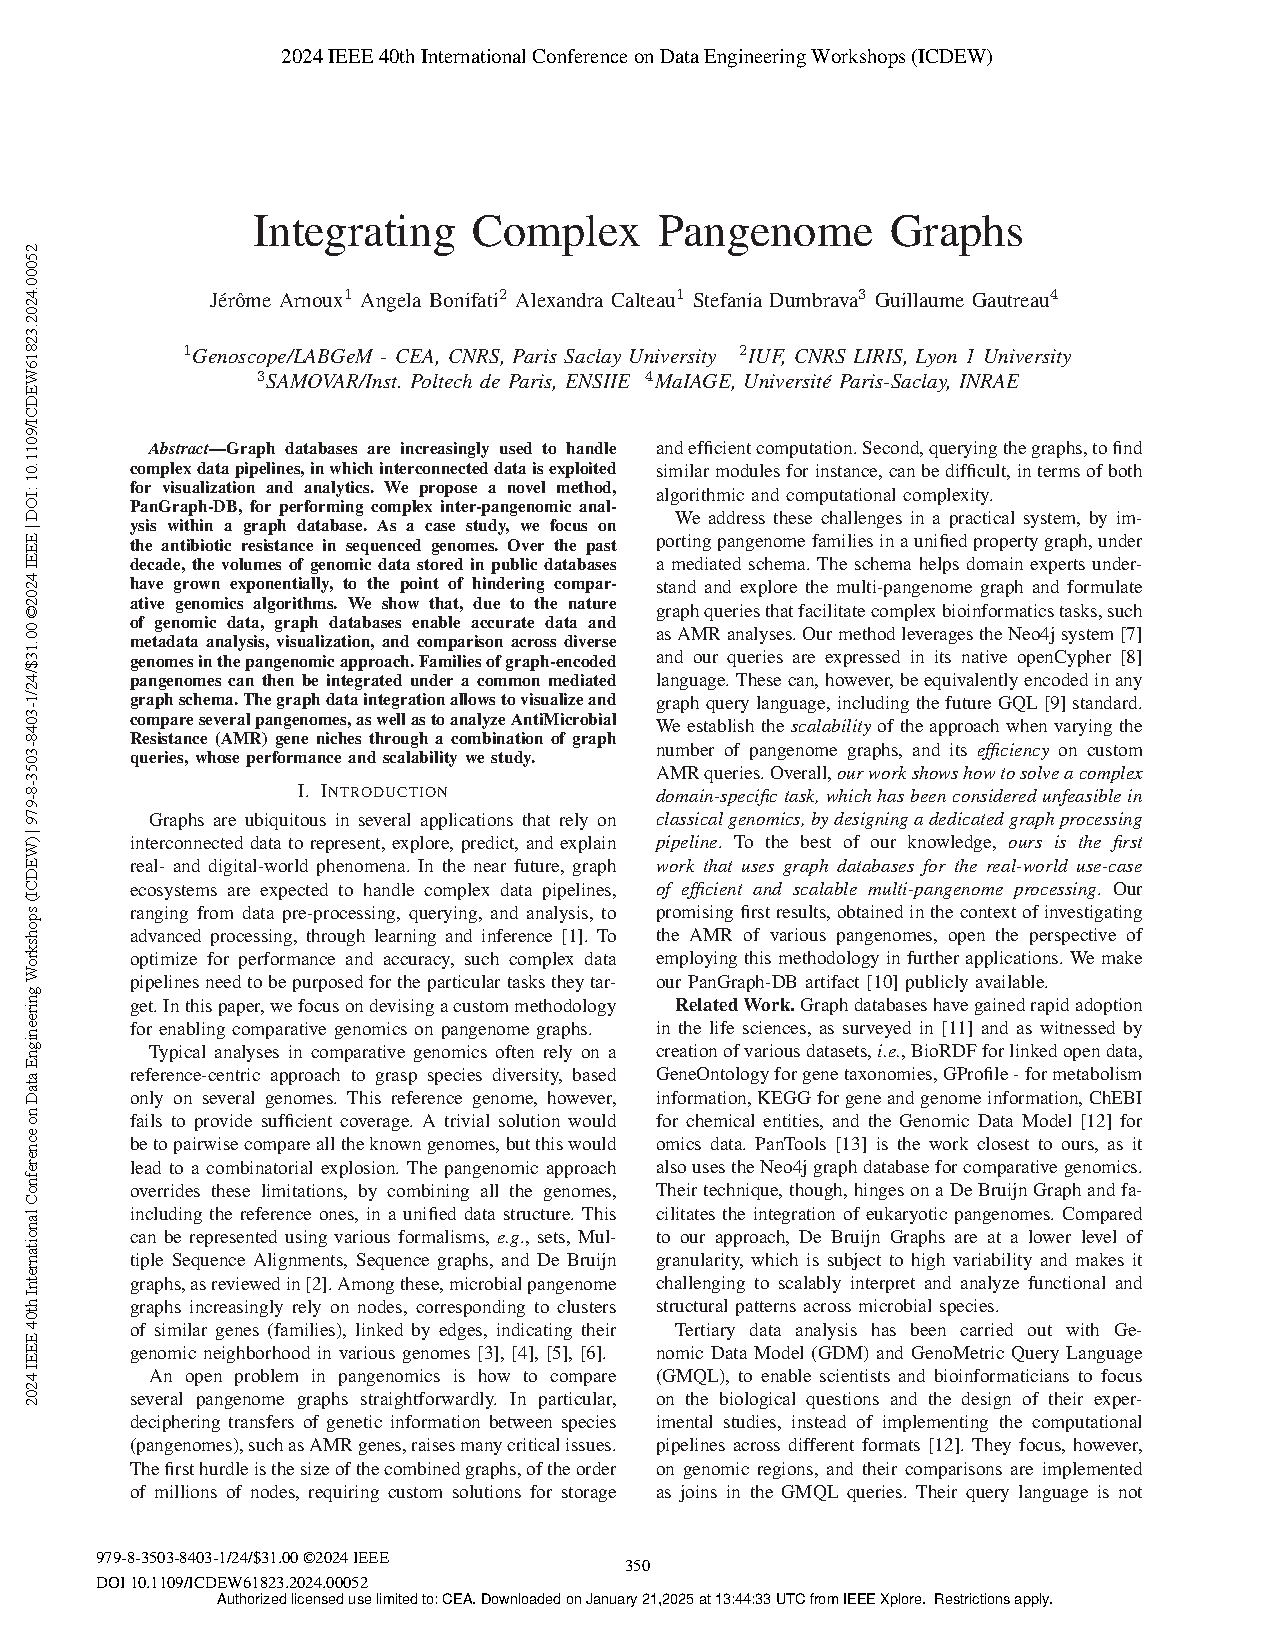
\includepdf[pages=-]{GraphDataBase/Integrating_Complex_Pangenome_Graphs.pdf}

\chapter{Conclusion et perspectives}

Notre \textit{proof of concept} sur l'intégration et l'analyse de pangénomes dans des bases de données orientées graphe, ouvre la voie à de nouvelles méthodes de stockage, d’analyse et de visualisation de vastes ensembles de génomes et de pangénomes. Nous avons conçu un schéma de base de données ainsi qu’un workflow d’analyse générique, pouvant être adaptés à d'autres modèles de pangénomes. Nos tests montrent que notre approche permet des temps de réponse très rapides (de l’ordre de la milliseconde) aussi bien pour des requêtes simples que pour des analyses complexes. Bien que notre POC soit une réussite, plusieurs améliorations sont nécessaires pour en faire une véritable base de données opérationnelle dédiée à l’analyse et à la distribution des pangénomes.

Pour intégrer les pangénomes dans la base de données, j'ai développé un script Python utilisant \textbf{PPanGGOLiN} et \textbf{PANORAMA} afin d’extraire et de préparer les données. L’intégration dans Neo4j s’est appuyée sur des packages tiers, non optimisés pour nos données, entraînant des temps d’intégration relativement longs. Récemment, Neo4j a publié un package officiel, plus flexible et optimisé pour la communication avec la base. Les premiers tests, que j'ai menés, indiquent qu’il permettrait une réduction significative des temps d’intégration, ce qui constitue une piste prometteuse pour améliorer l'efficacité globale du système.

Lors d’un second hackathon D4GEN en 2023, l’intégration de \textbf{méthodes de machine learning} a été explorée dans notre workflow d’analyse. Neo4j propose plusieurs packages dédiés à l’application du ML directement sur la base de données. Nous avons testé différentes approches pour identifier des structures et des chemins pertinents dans le graphe de pangénome, mais aucun résultat probant n’a émergé.
Cependant, cette première tentative nous a permis de repenser le schéma de la base de données et d'imaginer de \textbf{nouvelles métadonnées} à intégrer pour des analyses futures.

Pour construire la BD Neo4J, nous avons développé un script permettant de charger les pangénomes dans une base de données locale. Ce script avait d'abord été intégré à PANORAMA, pour sa capacité à lire plusieurs pangénomes. Toutefois, nous avons finalement choisi de développer un script indépendant, plus facile à maintenir. Ce script offre plusieurs avantages : intégration simplifiée des pangénomes dans la base, lancement automatique des analyses, indépendance vis-à-vis de l’interface Neo4j.
L’objectif étant de rendre l’ensemble du processus plus accessible et automatisé, afin que chacun puisse créer une instance propre de base de données de pangénomes.

Le \textbf{LABGeM} développe une base de données de pangénomes générés par PPanGGOLiN, \textbf{PanGBank}. Ce projet repose sur une architecture de BD relationnelle \textbf{SQL}, contenant les fichiers \textbf{HDF5} pour chaque espèce et des résultats d’analyse accessibles en ligne.
Une intégration avec notre POC pourrait offrir plusieurs avantages :
\begin{itemize}
    \item Une \textbf{nouvelle manière d’organiser et de visualiser les pangénomes}
    \item La possibilité d’\textbf{effectuer des analyses complexes directement sur la base de données}
    \item Une meilleure interconnexion entre les données et les outils d’exploration
\end{itemize}
En combinant ces approches, nous pourrions développer un système de gestion des pangénomes plus robuste, interactif et performant.
